\documentclass[aspectratio=169]{beamer}

% Pacote de estilo da UDESC
\usepackage{style/udesc}
\usepackage{listings}
\usepackage{hyperref}
\setbeamertemplate{itemize items}[circle]
\usepackage[abnt-emphasize=bf,abnt-and-type=e,alf]{abntex2cite}%Citações ABNT

% Incluir arquivos da pasta figuras
\graphicspath{{./img/}}


\setbeamertemplate{frametitle continuation}{}

% aPacote de texto aleatório
\usepackage{lipsum}

\lstset{ 
	basicstyle=\footnotesize,        % the size of the fonts that are used for the code
	breakatwhitespace=false,         % sets if automatic breaks should only happen at whitespace
	breaklines=true,                 % sets automatic line breaking
	captionpos=b,                    % sets the caption-position to bottom
	deletekeywords={...},            % if you want to delete keywords from the given language
	escapeinside={\%*}{*)},          % if you want to add LaTeX within your code
	extendedchars=true,              % lets you use non-ASCII characters; for 8-bits encodings only, does not work with UTF-8
	firstnumber=0,                % start line enumeration with line 1000
	frame=single,	                   % adds a frame around the code
	keepspaces=true,                 % keeps spaces in text, useful for keeping indentation of code (possibly needs columns=flexible)
	language=Java,                 % the language of the code
	morekeywords={*,...},            % if you want to add more keywords to the set
	numbers=none,                    % where to put the line-numbers; possible values are (none, left, right)
	numbersep=0pt,                   % how far the line-numbers are from the code
	rulecolor=\color{black},         % if not set, the frame-color may be changed on line-breaks within not-black text (e.g. comments (green here))
	showspaces=false,                % show spaces everywhere adding particular underscores; it overrides 'showstringspaces'
	showstringspaces=false,          % underline spaces within strings only
	showtabs=false,                  % show tabs within strings adding particular underscores
	stepnumber=2,                    % the step between two line-numbers. If it's 1, each line will be numbered
	tabsize=1,	                   % sets default tabsize to 2 
	basicstyle=\fontsize{7}{8}\selectfont\ttstyle,
	keywordstyle=\color{blue},
	commentstyle=\fontsize{7}{8}\selectfont\ttstyle\color{gray},
	stringstyle=\color{orange},
}
\tikzset{hide on/.code={\only<#1>{\color{white}}}}


% Início do documento
\begin{document}
\usetikzlibrary{positioning}
\usetikzlibrary{shadows.blur, trees}
\definecolor{greenudesc}{HTML}{01934A}



%%
%%	Incluir \capa para os slides
%% 
\titulo{Trilhas do Conhecimento}
\subtitulo{Sequência Didática\\EEB -- Giovani Pasqualini Faraco}
\newcommand{\autor}{Rodrigo Ribamar Silva do Nascimento}
\newcommand{\github}{github.com/physikices}
\newcommand{\email}{rodrigo.nascimento@edu.udesc.br}
\newcommand{\website}{}
\frase{2023 -- ECS4003}
\universidade{Universidade do Estado de Santa Catarina}
\capa

\AtBeginSection[]{
	\begin{frame}<beamer>
		\frametitle{Seções}
		\tableofcontents[currentsection]
\end{frame}}


\section{Trilha}
\subsection{Aspectos Gerais}
\subsection{Objetivos}
\subsection{Habilidades Vinculadas às Áreas de Conhecimento}

\section{Sequência Didática}
\subsection{Referenciais}
\subsection{Conteúdos Relacionados}
\subsection{Metodologia}
\subsection{Resultados}
% \subsection{Estrutura}
% \subsection{Cronograma de Aplicação}

\begin{frame}{Trilha}
	\framesubtitle{Aspectos Gerais}
	\imagem{trilha_ficahTecnica-01.png}{\cite{GPF_PE:2020}}
\end{frame}

\begin{frame}{Trilha}
	\framesubtitle{Aspectos Gerais}
	\begin{figure}[H]
		\tikzset{
			basic/.style  = {draw, text width=5em, rectangle},
			root/.style   = {basic,blur shadow={
					shadow blur steps=10,
					shadow blur extra rounding=2pt, 
					shadow xshift=1pt
			}, thin, align=center, fill=blue!45 , text width=30em},
			level 2/.style = {visible on=<2-7>, basic, thin, align=center, fill=green!30, text width=5em},
			level 3/.style = {visible on=<3-7>, rounded corners, thin, align=left, fill=cyan!20, text width=5em, node distance = 30pt},
			level 4/.style = {visible on=<4-7>, rounded corners, basic, thin, align=center, fill=red!20, text width=20em, node distance = 50pt},
		}

		\begin{tikzpicture}[
			level 1/.style={sibling distance=120pt},
			edge from parent/.style={visible on=<2-7>,->,draw},>=latex
			]
			\node[root, text=white] {\textbf{TRILHA\\(\emph{Modelagem de Fenômenos Naturais, Sociais e seus Impactos})} }
				child {node[level 2] (c1) {\textbf{UE01}}} 
				child {node[level 2] (c2) {\textbf{UE02}}}
				child {node[level 2] (c3) {\textbf{UE03}}};
			\begin{scope}[every node/.style={level 3}]
				\node [below of = c1, xshift=10pt] (c11) {Iniciação Científica};
				\node [below of = c11 ] (c12) {Processos Criativos};
				\node [below of = c12 ] (c13) {Med. e Int. Cultural};
				\node [below of = c13 ] (c14) {Empreed.};
			\end{scope}

			\begin{scope}[every node/.style={level 4}]
				\node [right of = c11, xshift=130pt, yshift=-30pt, visible on=<4>] (c11a) {
						\begin{itemize}
							\item Identificar, selecionar, processar e analisar dados com curiosidade [...]
							\item Posicionar-se com base em critérios científicos [...]
							\item Utilizar informação, conhecimentos [...] resultantes de investigação científica [...]
						\end{itemize}
					};
				\path (c11) edge [visible on=<4>, ->, draw] (c11a);

				\node [right of = c12, xshift=120pt, yshift=-10pt, visible on=<5>] (c12a) {
						\begin{itemize}
							\item Reconhecer e analisar diferentes manifestações criativas [...]
							\item Questionar, modificar e adaptar ideias existentes e criar propostas [...]
							\item Difundir novas ideias, propostas, [...] por meio de diferentes linguagens [...]
						\end{itemize}
					};
				\path (c12) edge [visible on=<5>, ->, draw] (c12a);

				\node [right of = c13, xshift=120pt, yshift=30pt, visible on=<6>] (c13a) {
						\begin{itemize}
							\item Reconhecer e analisar questões sociais, culturais e ambientais [...]
							\item Compreender e considerar a situação, a opinião e o sentimento do outro, agindo com empatia [...]
							\item Participar ativamente da proposição, implementação e avaliação de solução para problemas socioculturais e/ou ambientais [...]
						\end{itemize}
					};
				\path (c13) edge [visible on=<6>, ->, draw] (c13a);

				\node [right of = c14, xshift=120pt, yshift=70pt, visible on=<7>] (c14a) {
						\begin{itemize}
							\item Reconhecer e utilizar qualidades e fragilidades pessoais com confiança para superar desafios [...]
							\item Utilizar estratégias de planejamento, organização e empreendedorismo para estabelecer metas [...]
							\item Refletir continuamente sobre seu próprio desenvolvimento [...]
						\end{itemize}
					};
				\path (c14) edge [visible on=<7>, ->, draw] (c14a);
			\end{scope}

			\uncover<3-7>{
				\foreach \value in {1,2,3,4}
				\draw[->] (c1.195) |- (c1\value.west);
			}
		\end{tikzpicture}\\
	\end{figure}
\end{frame}

\begin{frame}{Trilha}
	\framesubtitle{Aspectos Gerais}
	\begin{columns}
		\column{0.5\textwidth}
		Ficha Técnica
		\begin{itemize}
			\item \textbf{Tema:} Modelagem de fenômenos naturais e sociais
			\item \textbf{Áreas de Conhecimento:} Todas (BNCC)
			\item \textbf{Carga Horária:} 160h
			\item \textbf{Aulas Semanais:} 10 aulas
		\end{itemize}

		\column{0.5\textwidth}
		Eixos Estruturantes e Habilidades Gerais:
		\begin{itemize}
			\item Investigação Científica
			\item Processos Criativos
			\item Mediação e Intervenção Sociocultural
			\item Empreendedorismo
		\end{itemize}
	\end{columns}
\end{frame}

\begin{frame}{Trilha}
	\framesubtitle{Aspectos Gerais}
	\begin{block}{Unidade Curricular 01:}
		Desastres naturais no território catarinense: impactos econômicos e sociais
	\end{block}
	\uncover<2->{
		\begin{block}{Unidade Curricular 02:}
			Desafio e possibilidades de (com)viver pós-pandemia no mundo do trabalho		
		\end{block}
	}
	\uncover<3->{
		\begin{block}{\textcolor{greenudesc}{Unidade Curricular 03:}}
			\textcolor{greenudesc}{A Natureza e sua força: fenômenos meteorológicos e seus impactos no mundo}
		\end{block}
	}
\end{frame}


\begin{frame}{Trilha}
	\framesubtitle{Aspectos Gerais}
	\begin{block}{Texto Introdutório da Trilha}
		Esta trilha de aprofundamento \alert<2->{trata da modelagem de fenômenos naturais e sociais} como chuva, tornados, deslizamentos, ciclos biogeoquímicos, desemprego, aumento na produção de riquezas, taxas de mortalidade, crescimento econômico, entre outros. A \alert<3->{modelagem, na educação básica, é um processo de ensino e aprendizagem que age de forma integrada com as diversas áreas do conhecimento}[...] \cite{GPF_PE:2020}
	\end{block}
\end{frame}

\begin{frame}{Trilha}
	\framesubtitle{Objetivos}
	\begin{block}{Objetivo da trilha de aprofundamento}
		Aprofundar conceitos das áreas de conhecimento por meio da modelagem de fenômenos naturais, sociais e seus impactos, construindo argumentação para a apropriação de conhecimentos científicos. \cite{GPF_PE:2020}			
	\end{block}
\end{frame}

\begin{frame}{Trilha}
	\framesubtitle{Habilidades Vinculadas às Áreas de Conhecimento}
	\begin{block}{Unidade Curricular 3}
		\only<1>{
			\begin{center}
				\textcolor{greenudesc}{{\large Descrição da Unidade}}
			\end{center}
			[..]serão apresentados objetos do conhecimento que \textbf{visam a contribuir com a ampliação do repertório científico} dos estudantes \textbf{para questões voltadas aos fenômenos naturais} que ocorrem \textbf{no estado de Santa Catarina}. Neste sentido, \textbf{o objetivo da unidade é estudar as questões sociais, culturais e ambientais de forma integrada entre todas as áreas do conhecimento} envolvidas na ocorrência dos fenômenos meteorológico no território catarinense e no mundo.
		}
		\only<2>{
			\alert{Investigação Científica}
			\imagem{trilha_UC01IC.png}{Fonte: \cite{GPF_PE:2020}}
		}
		\only<3>{
			\alert{Processos Criativos}
			\imagem{trilha_UC01PC.png}{Fonte: \cite{GPF_PE:2020}}
		}
		\only<4>{
			\alert{Mediação e Intervenção Sociocultural}
			\imagem{trilha_UC01MIS.png}{Fonte: \cite{GPF_PE:2020}}
		}
		\only<5>{
			\alert{Empreendedorismo}
			\imagem{trilha_UC01Emp.png}{Fonte: \cite{GPF_PE:2020}}
		}
	\end{block}	
\end{frame}

\begin{frame}[plain]
	\tikzset{
		udesc greenBox/.style = {
			thin,
			blur shadow={
				shadow blur steps=10,
				shadow blur extra rounding=2pt, 
				shadow xshift=1pt
			},
			rectangle,
			minimum width=75mm,
			minimum height=20mm,
			fill=greenudesc,
			text centered,
			anchor=base,
			inner sep=2ex
		},
	}
	\begin{tikzpicture}[remember picture,overlay]
		\node
			[udesc greenBox,yshift=-25pt,xshift=15pt] (box){}; 
		\node [right of = box, align=right,text=white] { {\LARGE Sequência Didática}\\Proposta};
	\end{tikzpicture}
\end{frame}

\begin{frame}{Sequência Didática}
	\framesubtitle{Referenciais}
	\begin{columns}
		\column{0.5\textwidth}
		\imagem{seq_mario}{SEI}

		\column{0.5\textwidth}
		\begin{itemize}
			\item \textbf{Autor:} Mario H. Calegari
			\item \textbf{Ano:} 2017
			\item \textbf{Turma:} 2° Ano EM (matutino)
			\item \textbf{Local:} EEB. Giovani Pasqualini Faraco
			\item \textbf{Orientadora:} Dra. Ivani T. Lawall
			\item \textbf{Coorientador:} Dr. Alex Bellucco do Carmo
			\item \textbf{Banca:} Dra. Lúcia H. Sasseron \& Dr. Carlos R. Rocha 
		\end{itemize}
	\end{columns}
\end{frame}

\begin{frame}{Sequência Didática}
	\framesubtitle{Conteúdos Relacionados}
	% Please add the following required packages to your document preamble:
	% \usepackage{graphicx}
	\begin{table}[ht!]
		\resizebox{.9\textwidth}{!}{%
			\begin{tabular}{|r|l|l|}
				\hline
				\multicolumn{1}{|c|}{\textbf{Aula}} & \multicolumn{1}{c|}{\textbf{Etapa (SEI)}} & \multicolumn{1}{c|}{\textbf{Atividade de Ensino}} \\ \hline
				01 & Contextualização & \begin{tabular}[c]{@{}l@{}}Vídeo: Mudanças Climáticas;\\ Pesquisa: O que influência a previsão\end{tabular} \\ \hline
				02 & Problematização & \begin{tabular}[c]{@{}l@{}}Apresentação da Pesquisa (Alunos)\\ Apresentação da SEI: Problemática (Previsão do tempo para a festa)\\ Apresentação da Estação Meteorológica\\ Montagem das Equipes\end{tabular} \\ \hline
				03 & Resolução dos Problemas & \begin{tabular}[c]{@{}l@{}}Organização da Coleta de Dados\\ Apresentação de Estratégias (Equipes)\end{tabular} \\ \hline
				04 & Atividade Investigativa & Condensação da Água \\ \hline
				05 & Atividade Investigativa & Pressão Atmosférica \\ \hline
				06 & Atividade Investigativa & Balão de Ar Quente \\ \hline
				07 & Resolução dos Problemas & \begin{tabular}[c]{@{}l@{}}Utilização dos Dado Coletados\\ Previsão do Tempo para os Próximos Dias\end{tabular} \\ \hline
				08 & Sistematização & Debate Sobre os Resultados \\ \hline
			\end{tabular}%
		}
		\caption{Fnte: \cite{MARIO:2017}}
	\end{table}

\end{frame}

\begin{frame}{Sequência Didática}
	\framesubtitle{Metodologia}
	\tikzset{
		basic/.style = {
			sibling distance=4.5cm,
			draw,
			rectangle
		},
		root/.style = {
			basic,
			align=center,
			fill=blue!75,
			text width=15em,
			blur shadow={
				shadow blur steps=10,
				shadow blur extra rounding=2pt,
				shadow xshift=1pt
			},
			thin,
		},
		level 1/.style = {
			basic,
			thin,
			align=center,
			fill=red!60,
			text=white,
			text width=11em
		},
		level 2/.style = {
			basic,
			thin,
			align=center,
			fill=green!30,
			text width=7em,
			text=black
		},
		level 3/.style = {
			basic,
			rounded corners,
			thin,
			align=center,
			fill=cyan!20,
			text width=9.5em
		}
	}
	\centering
	\begin{tikzpicture}
		\node[root, text=white] {Sequência de Ensino Investigativo\\Tema: Meteorologia}
			[edge from parent fork down]
			child [hide on=-1]{node[level 1, visible on=<2->] {Análise por Níveis de Engajamento}
				child [hide on=-2]{node[level 2, visible on=<3->] {\textbf{Nível-1:} Engajamento}
					child [hide on=-2]{node[level 3, visible on=<3->]{\textit{Indicador:} Discurso\\ Interesse/participação}}
				}
				child [hide on=-3]{node[level 2, visible on=<4->] {\textbf{Nível-2:} Engaj. Disciplinar}
					child [hide on=-3]{node[level 3, visible on=<4->]{\textit{Indicador:}\\ $E\xrightleftharpoons[transitividade]{}C$}}
				}
				child [hide on=-4]{node[level 2, visible on=<5->] {\textbf{Nível-3:} Engaj. Disciplinar Prod.}
					child [hide on=-4]{node[level 3, visible on=<5->]{\textit{Indicador:} Sofisticação da linguagem/Envolv. Emocional}}
				}
			};
		% child {node[level 2, visible on=<1->]  {Metakognition}
		%     child [hide on=-2]  {node {Planung}}
		%     child [hide on=-3] {node {Monotoring}}
		%     child [hide on=1] {node {Regulation}}}

	\end{tikzpicture}
\end{frame}

\begin{frame}{Sequência Didática}
	\framesubtitle{Metodologia}
	\begin{columns}
		\column{0.5\textwidth}
		\begin{figure}[htb!]
			\centering
			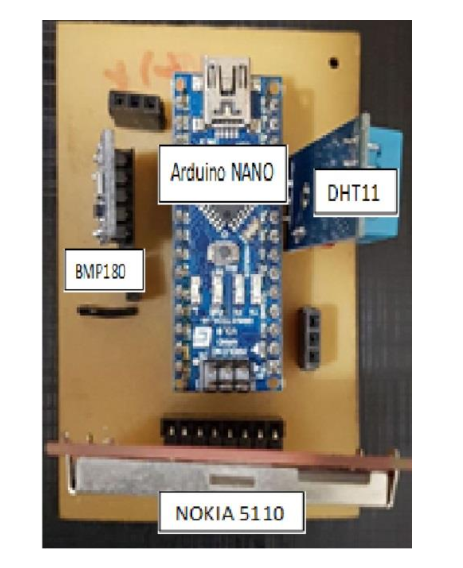
\includegraphics[width=.5\linewidth]{img/placa_arduino.png}
			\caption{\cite{MARIO:2017}}
		\end{figure}

		\column{0.5\textwidth}
		\begin{figure}[htb!]
			\centering
			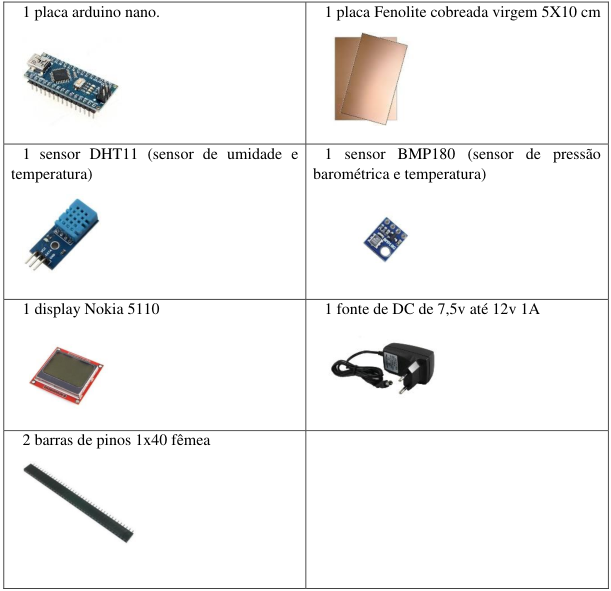
\includegraphics[width=.7\textwidth]{img/placa_arduino_cmpnts.png}
		\end{figure}
	\end{columns}
\end{frame}

\begin{frame}{Sequência Didática}
	\framesubtitle{Resultados}
	% Please add the following required packages to your document preamble:
	% \usepackage{graphicx}
	\begin{table}[]
		\resizebox{.8\textwidth}{!}{%
			\begin{tabular}{|r|l|l|l|l|l|}
				\hline
				\multicolumn{1}{|c|}{\textbf{Data}} & \multicolumn{1}{c|}{\textbf{Hora}} & \multicolumn{1}{c|}{$T(\unit{\degreeCelsius})$} & $U(\%)$ & $P(\unit{\hecto\pascal})$ & \textbf{Condic.} \\ \hline
				03/08 & 9h00 & 14,7 & 96 & 1024,7 &  \\ \hline
				04/08 & 9h00 & 16,4 & 96 & 1023,1 & Chuva \\ \hline
				05/08 & 9h00 & 17,9 & 95 & 1019,6 &  \\ \hline
				06/08 & 9h00 & 15,4 & 97 & 1014,6 & Chuva \\ \hline
				07/08 & 9h00 & 16,2 & 87 & 1018,7 & Chuva \\ \hline
			\end{tabular}%
		}
		\caption{Fonte: \cite{MARIO:2017}}
	\end{table}
\end{frame}


\begin{frame}[allowframebreaks]
	\frametitle{Referencias}
	\bibliography{referencias.bib}
\end{frame}

\contato{%
	Contato: \\
	\autor{} \\
	\email{} \\
	\github{} \\
	\website{}
}

\capadetras{}

\end{document}
